\documentclass[11pt]{article}

% ---- 预印本用最朴素的 arXiv 风格；投 workshop 时再换 sty ----
\usepackage[margin=1in]{geometry}
\usepackage[T1]{fontenc}
\usepackage{lmodern}
\usepackage{amsmath,amssymb}
\usepackage{graphicx}
\usepackage{booktabs}
\usepackage{hyperref}
\usepackage{natbib}
\usepackage{xcolor}
\usepackage{multirow}
\usepackage{siunitx}

\hypersetup{colorlinks=true,linkcolor=blue,citecolor=blue,urlcolor=blue}

% ---- paperkit 绑定宏（等价于 \input{audit/preamble}；内联以保证 clean clone 也能编） ----
\providecommand{\fact}[1]{}          % \fact{ID}：数字审计用，排版不产生字符
\providecommand{\pkignore}[1]{#1}    % 显式豁免区：内容照排，不进数字审计

\newcommand{\sys}{\textsc{Sih}}

% 草稿批注宏：终稿恒为空宏；待办统一收集在 human_todo.md
\newcommand{\todoq}[1]{}

\title{Deliver the Evidence, Not the Rules:\\
\large Context Compilation for Long-Horizon Coding Agents}
\author{Anonymous}
\date{\today}

\begin{document}
\maketitle

\begin{abstract}
Long-horizon coding agents are usually made stronger by giving them more context, as if the binding constraint were how much of a repository fits in the window.
We treat the prompt as a compiled artifact instead: typed sections under per-kind share budgets, a locator card that names where to look and which test failed, a ledger of what the model was actually shown, and mechanical gates that decide when the agent must stop revising and submit.
On a 16-instance\fact{A1} subset of SWE-bench Verified with DeepSeek V4.1 Flash, evidence delivery changed the resolve rate from 5/16\fact{A3} to 10/16\fact{A2} in a paired run where context assembly was the only variable.
On a single long task, six process constraints in the system prompt left MiniMax-M3.1-Flash at 0/3\fact{E5}; once the locator card was actually rendered and a mechanical cap allowed two patch versions, the same task closed at 5/5\fact{E8}.
Replaying those six tasks' recorded requests, our arm spent 73,051\fact{D2} output tokens per task against 12,495\fact{D2} for the official mcode CLI.
The scope is narrow: one model family per experiment, small task sets, one run per arm.
\end{abstract}

% FACTS-USED: A1, A2, A3, D2, E5, E8


\section{Introduction}

Long-horizon coding tasks ask an agent to enter an unfamiliar repository, find the cause of a failure, edit, and verify, often across dozens of tool calls.
The default response to failure is capacity: enlarge the window, retrieve more files, compact earlier turns less aggressively, let the agent search for longer.
Each of these assumes that the agent fails because the right material is missing from its prompt or too far away to keep.
That assumption held only partly in our runs.
More material helped, but not in proportion to how much we added, and several failures occurred with the relevant file already in the window: the agent read the failing test, then edited a different function.
The bottleneck we could measure was not how much context the model held, but whether the evidence it needed---where to look, what broke, and when to stop---reached it intact and in a form it could act on.

Our first observation is that direction beats volume.
We ran a paired comparison on a subset of SWE-bench Verified sized at 16 instances\fact{A1}, using DeepSeek V4.1 Flash and a single flag that turns context assembly on or off; task statements were copied verbatim, and the two arms differed in nothing else.
The assembly arm resolved 10/16\fact{A2}; the plain arm resolved 5/16\fact{A3}.
Two instances fail even with the gold patch here, so we also report the set without them: 10/14\fact{A4} against 5/14\fact{A5}, and 10/14\fact{A6} fail-to-pass tests repaired against 6/14\fact{A6}.
The paired outcomes are one-sided: all 5\fact{A7} discordant instances favored assembly and 0\fact{A7} favored the plain arm.
The gain is not uniform across difficulty: in the easiest stratum the two arms resolved 7/7\fact{A8} and 4/7\fact{A8}, in the middle stratum 2/5\fact{A9} and 1/5\fact{A9}, and in the hardest 1/2\fact{A10} and 0/2\fact{A10}.
Nor did it buy its result with volume: mean tokens per instance were 90,431\fact{A11} with assembly and 96,184\fact{A12} without, and because the per-instance pairs are mixed we read this as ``not more expensive'' rather than as a saving.

A second observation concerns instrumentation.
In an earlier ablation on one long task, the locator card was assembled, counted against its budget, and reported as delivered; it had never reached the model.
The renderer dropped the section, and a search of the recorded request bodies for the card's first line found nothing\fact{E9}.
Once the card was actually rendered, first reads landed in the gold region on 4/4\fact{E6} attempts, but only 1/4\fact{E6} resolved.
Knowing where to look is necessary and not sufficient.
We therefore stopped trusting the assembler's own log: every claim below about what the model saw is checked against the request body.

The third observation concerns stopping.
On the same long task with MiniMax-M3.1-Flash, six process constraints written into the system prompt left the resolve count at 0/3\fact{E5}, and per-round output grew rather than shrank.
Prose in the prompt was read and not followed.
Replacing it with a mechanical turn-level reminder produced a different failure: the agent began writing patches but kept producing new versions without declaring one final, 0/2\fact{E7}.
Only a harness rule that made a third revision impossible---at most two patch versions, then submit---closed the task at 5/5\fact{E8}.
Repairs aimed at capacity behaved the same way: evicting repeated reads still gave 0/3\fact{E2}, enlarging the per-kind share 0/3\fact{E3}, and raising the session token ceiling 0/2\fact{E4}.

The fourth observation concerns cost.
Replaying the recorded request bodies of both arms on the same six tasks with MiniMax-M3.1-Flash, we attributed every token.
Our arm emitted 73,051\fact{D2} output tokens per task against 12,495\fact{D2} for the official mcode CLI, while consuming 21,941\fact{D3} fresh input tokens against 52,996\fact{D3}.
The input side is cheaper for us and the output side is not, which reverses the intuition that a context-heavy harness pays for input.
The two cost accountings disagree, and we report both: if every input token is priced as fresh, our arm looks 3$\times$\fact{H1} more expensive, whereas on the actual bill the ratio is 1.66$\times$\fact{D1} (\$0.0486\fact{D1} against \$0.0292\fact{D1} per task).
Spend also concentrates in failure: successful tasks averaged 78,844\fact{D6} tokens, while two failing tasks contributed 70.9\%\fact{D6} of all output.
A single probe that lowered reasoning effort from high to low cut thinking tokens from 941\fact{D4} to 243\fact{D4}, which suggests that the output spend is a knob rather than a property of the task.

The effect is not peculiar to one model family.
On the same six tasks with MiniMax-M3.1-Flash our arm resolved 3/6\fact{C4}; the official CLI resolved 3/6\fact{C1} under its default cap of 24\fact{C1} steps, and 5/6\fact{C1} when that cap was raised to 60\fact{C1} steps.
The two did not solve the same tasks: ours repaired the pytest instance, the CLI the pylint one\fact{C7}.
What we press is narrower and, we think, more useful: the differences we can measure track what reached the model and when it was allowed to stop.

Three contributions follow.
First, a context compiler: the prompt is built rather than concatenated, with typed sections under per-kind share budgets, evidence cards generated from the failing test and the repository graph, and a ledger that records what was rendered.
Second, a controlled measurement of delivery: 10/16\fact{A2} against 5/16\fact{A3} in a paired run, and a cut-by-cut ablation in which prompt rules moved nothing while a mechanical gate moved the same model to 5/5\fact{E8}.
Third, a cost attribution on replayed requests: output rather than input tokens, failure rather than success, and a ratio we report under both accountings, 3$\times$\fact{H1} when all input is priced as fresh and 1.66$\times$\fact{D1} on the bill.

% FACTS-USED: A1, A2, A3, A4, A5, A6, A7, A8, A9, A10, A11, A12, C1, C4, C7, D1, D2, D3, D4, D6, E2, E3, E4, E5, E6, E7, E8, E9, H1

\section{Related Work}

Long-horizon software benchmarks moved evaluation from function-level synthesis to repository-level repair.
SWE-bench collected real GitHub issues together with the tests that decide whether a patch resolves them \citep{jimenez2024swebench}; SWE-agent argued that the agent-computer interface, and not only the model, determines what an agent can accomplish inside such a repository \citep{yang2024sweagent}; OpenHands packaged the same workflow as an extensible platform \citep{wang2024openhands}.
Adjacent lines extend the environment rather than the repository: WebArena and OSWorld place agents in front of realistic web and desktop state \citep{zhou2023webarena,xie2024osworld}, while AgentBench compares agents across a set of interactive environments \citep{liu2023agentbench}.
These benchmarks report end-to-end success and treat the scaffold as a design choice to be optimized.
A parallel engineering literature builds harnesses that search, edit and test in a loop; such systems are usually evaluated as end products, with the context policy treated as an implementation detail.
What reaches the prompt at each step, and whether it arrived at all, is rarely the object of measurement.
Our setting differs in two ways: we hold the scaffold fixed and vary only the assembled context, and we verify delivery against the recorded request body rather than against the assembler's own log.

A second line studies what a model can do with the context it is handed.
LongBench assembles long inputs across tasks and languages to measure comprehension at length \citep{bai2023longbench}, and RULER shows that the effective context of current models falls short of the advertised window \citep{hsieh2024ruler}.
The engineering response has been to keep more and retrieve better: summarize or compact earlier turns, rank candidate files by similarity to the issue, and re-inject whatever looks relevant.
These methods optimize the quantity and the relevance of material.
The failures we observed had a different shape: the file was present and the direction was missing---the agent read the failing test and edited a neighbouring function.
We therefore spend a fixed budget on evidence (a locator card naming the failing test and the region to read, together with the failure output) and on structure (typed sections with share caps, so that one kind cannot evict another), and we audit the rendered prompt rather than the ranker's output.
Compilation, in this sense, is a budgeting problem rather than a retrieval problem.
Retrieval is usually scored by whether the right span appears somewhere in the window, a criterion that our locator experiment separates from whether the agent then acted on it.

A third line concerns tool use and adherence to instructions.
ReAct interleaves reasoning with actions \citep{yao2022react}; Toolformer has models learn when to call APIs \citep{schick2023toolformer}; the $\tau$-bench family evaluates tool--agent--user interaction in domains that come with written policies and scores whether the agent follows them \citep{yao2024taubench}.
The lever in this literature is usually training or prompting: better exemplars, better reasoning traces, explicit rules in the system message.
Instruction-following benchmarks make a related assumption from the other side: they ask whether a model restates or obeys a stated rule, not whether the environment makes violation impossible.
In our runs the prompting lever was measurably weak.
Six process constraints written into the system prompt left the resolve count at 0/3\fact{E5}, while enforcement inside the harness---a turn-level mechanical reminder, then a cap on how many patch versions could be submitted---changed behaviour within one run.
That is the difference we press: compliance is an interface property, not an instruction.
A policy that cannot be violated is not the same object as a policy that has been stated, and only the former survived our ablations.

% FACTS-USED: E5

\section{System}

\subsection{The assembly surface}

We treat the context window as a compilation target, not a transcript buffer.
Every turn the runtime assembles an ordered set of typed sections and hashes the
result before the model sees it. The code does not decide what belongs in the
window; a signed data file does.

That file declares fifteen kinds of section: charter, task, intent, tool
definitions and results, skills, project rules, repository map, locator card,
snippets, history summaries, memory, handoff material, progress document and
intent history. Each kind declares its source, loading mode, trust level, share
of the turn budget, drop policy, verification, the largest unit it may inline,
pointer preview, and the tool that expands a pointer.

Two properties do the work. First, the budget has three levels: a per-turn
total, a share per kind, a cap per unit. Exceeding the unit cap does not
truncate text; it replaces the text with a pointer into an object store, and
the pointer must resolve. Exceeding the share drops the section and writes the
drop to the ledger. A task profile may re-weight shares, but they must still
sum to at most the total; the loader refuses the registry otherwise.

Second, the loading mode carries the argument. Resident kinds --- charter, task,
intent --- are always present. Search and lazy kinds enter only when a query
resolves and hits. Summary kinds carry references back to the original. Derived
kinds are recomputed at assembly time from this turn's evidence and compared
with the recorded derivation, so a card cannot be inherited from an earlier
turn and passed off as fresh.

Before the writer's first token, a preflight step runs the failing selector with
no model call and records the frames, the failing test function and the failure
excerpt, leaving the tree unchanged. Its purpose is not speed: the first
evidence in the window is produced and recorded by the runtime, so the model
cannot be shown a tool result the ledger lacks.

\subsection{Invariants, and what they stop}

The register names twenty-one invariants over the assembly, evaluated at the
entry and fail-closed: a violation rejects the turn rather than degrading it.
Five carry the delivery argument.

The typed-section invariant requires every section to have a declared kind and rejects an
unknown one at the entry. It stops a new category of text --- a pasted log, a
stack trace --- from entering the window because some code path found it
convenient. Without it the share budget is arithmetic over an open set: correct
as arithmetic, hollow as a guarantee.

The query-justification invariant requires inclusion to be justified by a resolvable query and
a match. It stops ``just in case'' context, and it makes inclusion falsifiable:
every section has an answer to the question of why it is there.

The pointer-substitution invariant turns a unit that exceeds its cap into a pointer with a
resolvable reference inside the object store. It stops one file from owning the
window, and it made the ablation legible: a runaway read could no longer
quietly consume the evidence budget, because eviction became a logged drop.

The drop-logging invariant requires a dropped section to be logged. It stops silent
truncation, the failure that would make the arm label false: a context-on arm
can decay into ``context on for the first few turns'' while still being called
context-on.

The payload-hash invariant requires the hash recorded for a turn to be the hash of the
payload the model actually received. It stops post-hoc reconstruction, and it
later exposed a delivery bug: the locator card was written and scheduled, but
never reached the request body (Section~\ref{sec:locator}).

These five are not enforced with equal strength: some are checked structurally,
against the shape of a derivation, some semantically, against whether its
entries hold. We report the difference rather than rounding it away, because an
invariant documented as stronger than it is behaves like no invariant at all.

\subsection{Task classes}

The first runtime knew one kind of work: fix this bug, run the tests, accept or
reject. A task class is now a row in a data file with three fields. The plan
gives the step order and the prompts. The profile gives the budget shares;
long-horizon work moves budget from the repository map and the skill
descriptions into tool results, because there the bottleneck is remembering
what was read, not learning what tools exist. The gate is looked up
in a small registry: tests pass on the model's own report, node-level pass over
an externally supplied selector, or a command whose exit status decides and
whose output summary enters the evidence.

The point is not configurability: the SWE-bench runs are graded by node, with
the selector taken from the dataset. A new class costs a row, not a branch. The
loader refuses unknown fields, plans, profiles and gates, and an absent table
falls back to old behavior, so the abstraction cannot quietly change the
control arm. Our tool-and-policy experiments reuse the assembly surface through
a separate adapter that does not run the plan engine; we state that boundary
rather than paper over it.

\subsection{The accounting surface}

Every assembled turn has a canonical form and a hash; the rendered body is kept
in an object store, and the ledger keeps the hash and the reference, not the
text. The ledger therefore records what was delivered, not what was intended. A
turn that was assembled but never delivered appears as a gap, not a
plausible-looking row.

The execution layer adds epochs. The table of tool plates --- which tools exist,
with declared effect and risk --- is hashed into an epoch; reports carry the
epoch, and counts are never summed across epochs. Changing one line of that
table yields a new epoch, which guards against a measurement improving because
the thing measured changed underneath it.

For the experiments the consequence is narrow. The two arms differ by a single
switch; preflight, the gate, the close-out rule and the accounting are common
to both. The accounting surface is what lets us assert that without relying on
our memory of the runs.

% FACTS-USED: E9 (locator card never reached the request body)

\section{Mechanisms}

The four mechanisms answer four different questions: where to look, what the
failure means, when to stop, and what the run cost. Each is stated with the
observation that would falsify it, because the parts that were easiest to
describe were the parts most likely to be doing nothing.

\subsection{The locator card}
\label{sec:locator}

\paragraph{Motivation.} The long-horizon runs did not fail for lack of
information; they failed while reading. In the baseline the agent reopened the
same file repeatedly, never wrote a patch, and exhausted its rounds. It lacked
position: the failing test names a module, the seeded frame names a function
that merely calls the culprit, and the function to edit sits a short distance
away in the module's reference graph.

\paragraph{Approach.} Preflight yields the frames of the failing test with no
model call. One-hop entries are the symbols those frames name; two-hop entries
come from a breadth-first walk over a graph built from the module's abstract
syntax tree, with top-level functions, classes and module-level assignments as
nodes and name references inside bodies as edges. Candidates are ranked by task
words in the symbol name, then match strength, hop count and definition line.
The first three become cards carrying path, symbol, line span and a reason from
a closed set.

\begin{verbatim}
entries  <- symbols named by the failing frames
frontier <- entries
repeat at most twice:
    add top-level symbols referenced from frontier (in-module AST)
rank by (-task words in name, match tier, hop, line)
emit the first three entries as cards
\end{verbatim}

\paragraph{Criterion.} The card is judged by the first read. When it was first
delivered, the first read landed in the golden region on 4 of 4\fact{E6}
instances, and 1 of 4\fact{E6} resolved --- a mechanism check on four instances
of one task. The card names locations and never assertions: no test name, no
expected value, so it can point at the right function without handing over the
answer.

\paragraph{Failure modes.} The walk stays inside one module: cross-file calls
are not chased, types are not resolved, dynamic dispatch is invisible, and a
culprit reachable only through a package alias degrades the ranking to
structural order. The sharpest failure is delivery: for a sequence of arms the
card was computed and scheduled, yet a search of the stored request bodies for
the symbol it named found nothing\fact{E9}. A correct card that never
arrives is indistinguishable, from the outside, from a wrong one.

\subsection{Failure-test evidence}

\paragraph{Motivation.} An issue report describes a symptom; a test states a
contract. For the tabulate formatting issue the contract is a literal expected
string in which whitespace and quoting are part of the specification, so a patch
that satisfies the prose can still fail the assertion. Passing the whole test
file is the wrong repair: the window fills with unrelated cases, and the
editable file invites fixing the test instead of the code.

\paragraph{Approach.} The raw runner output is parsed for the innermost
test-side frame, and that line is mapped with the parser to the enclosing test
function, so the unit is the full definition rather than a fixed window. The
failure excerpt from the error block is appended and bounded. The result enters
as one ordinary tool-result section under the existing share: no extra budget,
no new kind. The ledger keeps the path, the
symbol, the span and an artifact reference; the text stays in the object store.
If preflight is green nothing is emitted, and the section reaches the model only
if the assembler placed it, so a section evicted by the share disappears from
the request rather than only from the ledger.

\paragraph{Criterion.} Containment. On the real instance the unit held the
failing function and its assertion excerpt and none of the other tests in the
same file; a unit test asserts their absence from both fields, and a switch
disables the injection for a separate measurement.

\paragraph{Failure modes.} Import and collection errors carry no assertion, so
only the frame survives. The culprit may be a helper one call below the test:
the locator reaches it, the evidence section does not, and the two mechanisms
disagree. A patch can be fitted to the literal and still regress tests
elsewhere, which is why acceptance is node-level. And the excerpt is raw runner
text, so a format change yields an empty payload that looks exactly like a task
with nothing to inject.

\subsection{Mechanical gates}

\paragraph{Motivation.} The gates answer a different question from context: not
what the model knows, but when the episode ends. Given the card and the failing
test, the agent often had what it needed and still did not stop. Instructions we
could write down were about behavior, and behavior is what a prompt is worst at
changing.

\paragraph{Prompt versus mechanism.} We first wrote the required process as six
constraints --- deliver a patch early, do not re-read a span, note a conclusion
before acting, stay in scope, hand in rather than test, keep output short ---
and assembled them as resident project-rule sections, ordered after the charter
and before the task, rendered into the system message. This is the obvious
implementation, and it did nothing: 0/3\fact{E5}. Per-turn output grew rather
than shrank, as though the rules had been read as a description of the
situation rather than a procedure.

Moving the same requirement into the loop changed behavior but not outcome.
From the seventh round, if no patch had been submitted, the runtime appended a
user-message reminder on every turn; patches appeared, but the model revised
instead of submitting: 0/2\fact{E7}.

Only when the runtime took the decision away did the task resolve. The step
allows at most two patch versions; on the second it closes, the last version
goes to the verifier, and the model is not asked whether it is done. Same task,
same model: 5/5\fact{E8}.

\paragraph{The symptom trap.} The pattern is not specific to rules. Removing
visible symptoms one at a time did not move the outcome: deduplicating repeated
reads 0/3\fact{E2}, enlarging the share available to file reads 0/3\fact{E3},
raising the token ceiling 0/2\fact{E4}. Each cut tidied the transcript and left
an episode that could not terminate; the starting point, with neither card nor
gate, was 0/3\fact{E1}.

\paragraph{Criterion.} The gate is judged by termination, not compliance: did
the episode close with a decision the verifier could judge. Compliance is
unobservable in a transcript the model writes; termination is an event in the
ledger, with a timestamp and a patch attached.

\paragraph{Failure modes.} The two-version cap can end an episode whose first
direction was wrong; in this sample it did not, but it is a designed way to
fail. The gate does nothing for a model that already converges: the DeepSeek
runs submit early enough that the reminder never fires.

\subsection{Cost accounting}

\paragraph{Motivation.} The ledger used to record one number per call: total
tokens. Providers bill three things differently --- fresh input, cached input,
and output, mostly invisible thinking --- and one total makes the cheap part
and the expensive part indistinguishable. Two agents with different caching
then look comparable when they are not.

\paragraph{Approach.} We record the provider's usage fields verbatim: prompt,
completion, cached prompt, reasoning. Absent fields are recorded as zero, never
inferred; the old total keeps its meaning, so earlier ledgers replay. Because
the rendered request body is stored per call, we can also replay the bodies with
a minimal output cap, read the real prompt size and cache hit of every turn, and
subtract to recover completion.

\paragraph{What the attribution shows.} The gap is in output, not in input:
average output is 73,051\fact{D2} tokens against 12,495\fact{D2} for mcode,
while fresh input is 21,941\fact{D3} against 52,996\fact{D3}. On the same six
tasks with the same model and endpoint the real bill is \$0.0486\fact{D1} per
task against \$0.0292\fact{D1}, a ratio of 1.66\fact{D1}. The familiar claim
that we are 3\fact{H1} times more expensive is the uncached accounting, which
charges every input token as fresh; failures also concentrate the spend, with
successful tasks averaging 78,844\fact{D6} tokens and two failed tasks
accounting for 70.9\%\fact{D6} of all output.

\paragraph{Criterion.} A cost claim must be recomputable from the ledger and a
public price list; when two conventions disagree, both are printed next to the
claim. The lever that follows is stopping, not compressing.

% FACTS-USED: E1, E2, E3, E4, E5, E6, E7, E8, E9, D1, D2, D3, D6, H1

\section{Evaluation}

We ask four questions. Does delivering evidence change outcomes on repository repair? Does the change survive a different difficulty mix? How does the arm compare with a mature command-line agent on the same tasks? And does anything transfer to a domain where the task is a written policy rather than a test? Each question has its own run; runs with different task sets, models or budgets are never pooled.

\subsection{Setting}

The main comparison uses a subset of SWE-bench Verified \citep{jimenez2024swebench} of 16\fact{A1} instances. The subset was not drawn at random. Every instance had already been checked, in an earlier batch on this machine, to fail before a patch and pass after the gold patch. That filter removes instances whose tests are broken here, and it also removes instances that are green from the start; the subset is therefore easier than a random draw of the benchmark, a point we return to in Section~\ref{sec:threats}.

Both arms ran DeepSeek V4.1 Flash with the same plan, the same preflight, the same node-level gate and the same close-out rule. The only difference is one flag that turns context assembly on or off. The task statement was copied verbatim from the dataset field, with no rewriting and no hint, and both arms received that same text.

Judging is node-level and external. We run the test selector shipped with the instance and count an instance resolved only when every fail-to-pass node passes and no pass-to-pass node regresses. The second clause does real work. A patch that repairs the reported failure while breaking a test that used to pass is not a repair, and in this batch one such run is present: the target node went green, a pass-to-pass node went red, and the instance is scored unresolved. It appears in Table~\ref{tab:main} as a row where the arms differ by that regression rather than by the target test.

Two instances fail even with the gold patch: the same pass-to-pass nodes fail on this machine whatever the model writes, because they depend on the shape of the local \texttt{sys.path}. We therefore report both denominators. Over all instances the arms resolved 10/16\fact{A2} and 5/16\fact{A3}. After removing the two baseline-red instances the counts are 10/14\fact{A4} and 5/14\fact{A5}, and the fail-to-pass count over the same 14\fact{A6} instances is 10/14\fact{A6} against 6/14\fact{A6}; the gap between that and the resolved count is the pass-to-pass clause above.

Table~\ref{tab:main} lists every instance, both arms and per-instance tokens; the baseline-red rows are marked and excluded from the headline. Table~\ref{tab:difficulty} splits the remaining 14\fact{A4} instances by the difficulty label shipped with the dataset.

\subsection{Main result}

Assembly resolved 10/16\fact{A2} and the plain arm 5/16\fact{A3}. The margin is less informative than its structure. Five instances are discordant, all five in favour of assembly and none in the other direction\fact{A7}. The remaining pairs agree, and in those the arms differ only in what they spent.

Spending does not explain the result, and it does not follow it either. Mean tokens per instance were 90,431\fact{A11} with assembly and 96,184\fact{A12} without; the medians were 85,928\fact{A11} and 95,655\fact{A12}, and mean calls were 14.8\fact{A13} and 15.6\fact{A13}. The per-instance pairs are mixed, so we read this as ``not more expensive'' rather than as a saving.

By difficulty, the direction is consistent and the absolute rates are not. In the easiest bucket, tasks labelled under fifteen minutes, assembly resolved 7/7\fact{A8} against 4/7\fact{A8}; in the middle bucket 2/5\fact{A9} against 1/5\fact{A9}; in the hardest 1/2\fact{A10} against 0/2\fact{A10}. The hardest bucket holds two instances, so its split carries no weight beyond direction. Table~\ref{tab:difficulty} also shows that assembly was cheaper in the easy bucket and more expensive in the middle one, which is why we report cost per bucket rather than one average.

The main run was preceded by a pilot on six of the same tasks with the same model. There assembly resolved 5/6\fact{B1} and the plain arm 4/6\fact{B1}, with one genuine difference: \pkignore{sphinx-10449} was repaired by the assembly arm at 210.8k\fact{B3} tokens and not by the plain arm at 104.2k\fact{B3}. The pilot's token means were 97.3k\fact{B2} against 84.7k\fact{B2}; its task set differs from the sixteen-instance set, so we do not pool the two means\fact{H2}.

% 生成件：勿手改。整表进 \pkignore 显式豁免区（见正文 \input 附近的 \fact 复述）。
\pkignore{%
\begin{table}[t]
\centering
\footnotesize
\setlength{\tabcolsep}{4pt}
\caption{SWE-bench Verified subset: resolved vs not, per instance. Baseline-red rows fail even with the gold patch and are excluded from the headline numbers.}
\label{tab:main}
\begin{tabular}{lrrrrr}
\toprule
Instance & Baseline-red & On & Off & On tokens & Off tokens \\
\midrule
pallets\_flask-5014 &  & \checkmark & \checkmark & 26,286 & 53,271 \\
psf\_requests-6028 &  & -- & -- & 82,105 & 64,375 \\
pylint-dev\_pylint-4970 &  & \checkmark & -- & 63,727 & 92,683 \\
pylint-dev\_pylint-6528 & yes & -- & -- & 136,118 & 147,369 \\
pylint-dev\_pylint-7277 & yes & -- & -- & 47,704 & 45,560 \\
pylint-dev\_pylint-8898 &  & \checkmark & -- & 126,537 & 98,627 \\
pytest-dev\_pytest-10051 &  & -- & -- & 56,742 & 76,973 \\
pytest-dev\_pytest-10081 &  & \checkmark & -- & 88,368 & 80,854 \\
pytest-dev\_pytest-10356 &  & -- & -- & 116,106 & 119,415 \\
pytest-dev\_pytest-7982 &  & \checkmark & \checkmark & 28,477 & 63,349 \\
pytest-dev\_pytest-8399 &  & \checkmark & \checkmark & 83,489 & 83,886 \\
sphinx-doc\_sphinx-10323 &  & \checkmark & \checkmark & 100,485 & 105,737 \\
sphinx-doc\_sphinx-10435 &  & \checkmark & \checkmark & 64,677 & 130,547 \\
sphinx-doc\_sphinx-10449 &  & \checkmark & -- & 119,770 & 110,119 \\
sphinx-doc\_sphinx-10614 &  & -- & -- & 169,853 & 153,599 \\
sphinx-doc\_sphinx-10673 &  & \checkmark & -- & 136,456 & 112,573 \\
\bottomrule
\end{tabular}

\par\smallskip\footnotesize resolved = all FAIL\_TO\_PASS nodes pass and no PASS\_TO\_PASS regression. Baseline-red marks the instances whose gold patch fails on this machine; one flaky gold run is not counted as baseline-red. Per-instance tokens come from the original batch report; later reruns of several instances are not reflected here.
\end{table}
}

% 生成件：勿手改。整表进 \pkignore 显式豁免区（见正文 \input 附近的 \fact 复述）。
\pkignore{%
\begin{table}[t]
\centering
\caption{Resolved count by dataset difficulty bucket, excluding the two stable baseline-red instances.}
\label{tab:difficulty}
\begin{tabular}{lrrrrr}
\toprule
Difficulty & n & On resolved & Off resolved & On tokens & Off tokens \\
\midrule
<15 min fix & 7 & 7/7 & 4/7 & 70,256 & 90,937 \\
15 min - 1 hour & 5 & 2/5 & 1/5 & 105,729 & 98,281 \\
1-4 hours & 2 & 1/2 & 0/2 & 121,322 & 109,021 \\
\bottomrule
\end{tabular}
\end{table}
}


\subsection{Against a mature CLI}

Table~\ref{tab:cost} compares two scaffolds on the same six tasks with MiniMax-M3.1-Flash. Under its default cap of 24\fact{C1} steps the official mcode CLI resolved 3/6\fact{C1}. When the cap was raised to 60\fact{C1} steps, the two instances that had produced empty patches were repaired and the count became 5/6\fact{C1}. These are two settings rather than a range: the first is a protocol arm, the second a rerun, and the difference is the step budget, not the model\fact{H3}.

Our arm on the same six tasks resolved 3/6\fact{C4}. It spent 195,228\fact{C5} tokens per task on average, 96,961\fact{C5} input and 98,267\fact{C5} output, where the output figure is recovered by subtraction and the input figure is itself an estimate; we record that fact as medium confidence. mcode spent 65,492\fact{C2} tokens per task, 52,996\fact{C2} input and 12,495\fact{C2} output. Wall time ran the other way: 480.9\fact{C6} seconds for our arm against 131\fact{C3} seconds for mcode, measured while two batches shared one provider key.

The two scaffolds did not solve the same instances: ours repaired pytest-10081\fact{C7}, mcode repaired pylint-8898\fact{C7}. The comparison places the arm in the same band as a mature CLI on this task set.

On the replayed requests the bill is \$0.0486\fact{D1} per task for our arm against \$0.0292\fact{D1} for mcode, a ratio of 1.66\fact{D1}; the 3\fact{H1} figure that circulated in our earlier accounting prices every input token as fresh and is not the bill. We print both because the two conventions support opposite sentences about the same run.

% 生成件：勿手改。整表进 \pkignore 显式豁免区（见正文 \input 附近的 \fact 复述）。
\pkignore{%
\begin{table}[t]
\centering
\caption{Same six SWE-bench tasks, same model (MiniMax-M3.1-Flash), two scaffolds.}
\label{tab:cost}
\begin{tabular}{lrrr}
\toprule
Scaffold & Resolved & Tokens/run & Wall time/run \\
\midrule
mcode (24-step cap) & 3/6 & 65,492 & 131s \\
mcode (60-step cap) & 5/6 & -- & -- \\
\sys{} (ours) & 3/6 & 195,228 & 480.9s \\
\bottomrule
\end{tabular}

\par\smallskip\footnotesize Resolved counts: C1 (mcode) and C4 (ours). Tokens and wall time: C2, C3, C5, C6. The 60-step row is a rerun under a raised cap; its tokens and time were not recorded. Our input/output split is an estimate; wall times come from two concurrent batches sharing one key.
\end{table}
}


\subsection{Across domains}

Table~\ref{tab:tau2} reports a tool-and-policy benchmark from the $\tau$-bench family \citep{yao2024taubench}, where success depends on following a written policy as well as calling tools correctly. In the retail domain our arm scored 0.900\fact{F1} against 0.800\fact{F1} for the reference agent, at 133,558\fact{F2} tokens against 113,602\fact{F2}, or 17.6\%\fact{F2} more. The run is ten tasks and a single trial, so a difference of this size is within noise. In the mock domain we scored 0.6\fact{F3} against 1.0\fact{F3}. Those failures were not policy violations: our agent passed a parameter object with an extra field, and the database rejected the call on a hash check. That is schema conformance, which the assembly surface does not address. For scale, a reference sample of the same benchmark scored 1.0\fact{F4} in 28.08\fact{F4} seconds at 94,568\fact{F4} tokens.

We also audited a container benchmark, Terminal-Bench, but only for environment health. Of 66\fact{G1} tasks reached, the oracle patch resolved 35/47\fact{G2} judged instances, 53\%\fact{G2} of the full set, at 507\fact{G4} seconds per task on average and 2220\fact{G4} seconds for the slowest. We report this as a ceiling on what any agent could score in our harness, not as an agent result.

% 生成件：勿手改。整表进 \pkignore 显式豁免区（见正文 \input 附近的 \fact 复述）。
\pkignore{%
\begin{table}[t]
\centering
\caption{Tool-and-policy benchmark ($\tau^2$-bench): reward and token cost.}
\label{tab:tau2}
\begin{tabular}{lrrrr}
\toprule
Domain & \sys{} reward & Reference reward & \sys{} tokens & Reference tokens \\
\midrule
retail (10 tasks) & 0.900 & 0.800 & 133,558 & 113,602 \\
mock (5 tasks) & 0.600 & 1.000 & -- & -- \\
\bottomrule
\end{tabular}

\par\smallskip\footnotesize Single trial per task; differences of this size are within noise.
\end{table}
}


\begin{figure}[t]
\centering
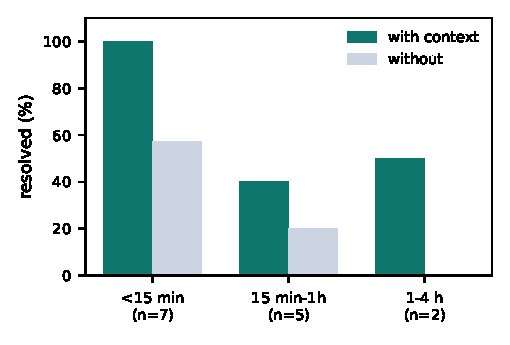
\includegraphics[width=0.55\linewidth]{figures/f2_swebench.pdf}
\caption{Resolved rate by dataset difficulty bucket, with and without context compilation.
Sample sizes are shown under each bucket; two baseline-red instances are excluded.
Data: Table~\ref{tab:difficulty} and the fact ledger.}
\label{fig:swebench}
\end{figure}

\begin{figure}[t]
\centering
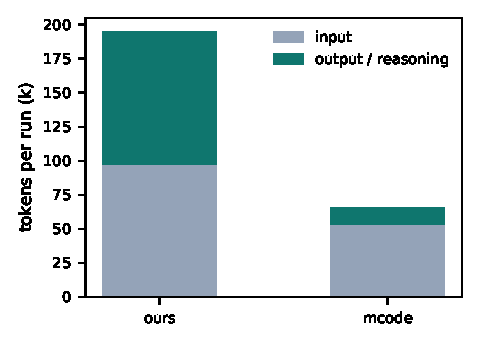
\includegraphics[width=0.55\linewidth]{figures/f3_cost.pdf}
\caption{Token composition per run for the two scaffolds on the same six tasks and model.
The gap is dominated by output (reasoning) tokens rather than by prompt size.
Data: the per-arm token accounting reported above.}
\label{fig:cost}
\end{figure}

% FACTS-USED: A1, A2, A3, A4, A5, A6, A7, A8, A9, A10, A11, A12, A13, B1, B2, B3, C1, C2, C3, C4, C5, C6, C7, D1, F1, F2, F3, F4, G1, G2, G4, H1, H2

\section{Ablations}
\label{sec:ablation}

The ablation asks a narrower question than the main comparison: on a single long task that the baseline never closes, which change makes closure possible? All arms use MiniMax-M3.1-Flash on the same tabulate formatting issue, on one machine with one key, run in sequence. We organise the result as four hypotheses; Appendix~\ref{app:debuglog} reproduces the run order and the per-arm cost of each step.

\paragraph{Hypothesis one: capacity.} If the episode fails because it runs out of room, then removing the pressure should let it finish.
We made three capacity interventions in turn: evicting repeated reads, raising the share of the budget available to file reads, and raising the session token ceiling.
The observations did not move. Deduplicating repeated reads left the count at 0/3\fact{E2}; enlarging the read share left it at 0/3\fact{E3}; raising the ceiling left it at 0/2\fact{E4}.
The starting point, with the card assembled but not delivered and with no gate, was 0/3\fact{E1}.
Each intervention removed a defect in the transcript and left an episode that could not terminate, so capacity was not the variable.

\paragraph{Hypothesis two: instruction.} If the episode fails because the model does not know the procedure, then stating the procedure should fix it.
We wrote the required process as six constraints --- deliver a patch early, do not re-read a span, note a conclusion before acting, stay in scope, hand in rather than test, keep output short --- and assembled them as resident project-rule sections, ordered after the charter and before the task, rendered into the system message.
The count stayed at 0/3\fact{E5}, and per-turn output grew rather than shrank.
The rules were read and treated as a description of the situation rather than as a procedure: adding text to the system prompt changed what the model said about its work, not what the episode did.

\paragraph{Hypothesis three: delivery.} If the evidence is correct but never arrives, then rendering it should move the first read.
We had reported the card as delivered; verifying the recorded request bodies showed that it had not been. Once the card was actually rendered, the first read landed in the gold region on every attempt, and the count moved to 1/4\fact{E6}.
The intervention solved direction and did not solve termination. It also separated delivery from effect: the card is necessary and, on this task, not sufficient.

\paragraph{Hypothesis four: the location of the decision.} If the model will not submit on its own, then the harness should take the decision away.
Moving a reminder into the loop produced patches but no submission: 0/2\fact{E7}. Capping the number of patch versions at two, closing on the second and sending the last version to the verifier, moved the count to 5/5\fact{E8}.
What separates this arm from the ones above is neither more evidence nor a better instruction but the location of the decision: the harness, not the model, decides when the episode ends.

Read as a sequence, the ablation is not a dose-response curve. The early arms each removed a visible defect and left the episode unable to close; the last arm removed a choice. That is why we treat the card as a precondition for the gate rather than as the intervention by itself, and why the mechanism claim is about the gate rather than about the amount of context.

\begin{figure}[t]
\centering
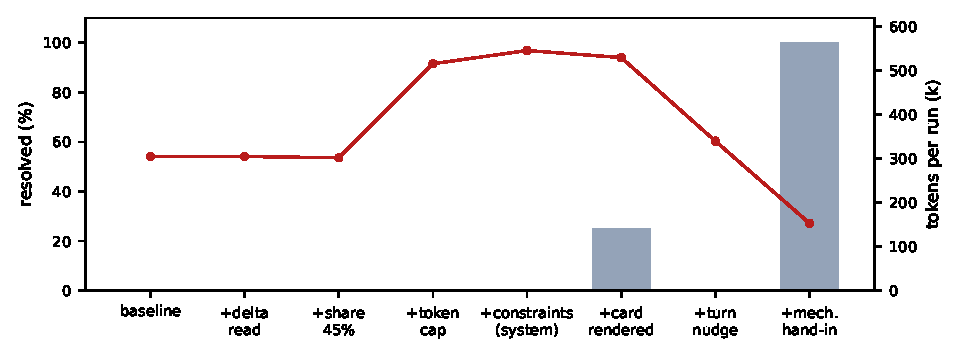
\includegraphics[width=\linewidth]{figures/f1_progression.pdf}
\caption{Incremental ablation on a single task (one tabulate issue, MiniMax-M3.1-Flash).
Each step adds one mechanism: repeated-read deltas, a larger tool-result share, a larger
session budget, prompt-level constraints, an actually-rendered locator card, a mechanical
turn nudge, and mechanical hand-in. Resolved count is the bar; tokens per run the line.
Data: Table~\ref{tab:ablation}; the run order is in Appendix~\ref{app:debuglog}.}
\label{fig:progression}
\end{figure}

% FACTS-USED: E1, E2, E3, E4, E5, E6, E7, E8

\section{Threats to Validity}
\label{sec:threats}

We separate limitations we know about and have not fixed, claim boundaries that follow from the size of the runs, and limitations that follow from the design.

\subsection{Known and not fixed}

The main comparison has 16\fact{A1} instances, 14\fact{A4} of them judgeable. A paired difference on that many cases has a wide interval, and we did not compute one; the direction of the 5\fact{A7} discordant pairs is more robust than the size of the margin. The cross-scaffold comparison is six tasks, the ablation one task, and every rate in this paper inherits that width.

Each experiment ran in a single window on a single machine, with one provider key per model and one run per arm. Arms ran in sequence, so provider drift and our own edits between arms are confounded with the variable under test. The ablation is the most exposed: it ran on one day with one key, its arms were not repeated, and its rows are a design history rather than a set of effect sizes. The last arm's 5/5\fact{E8} is five runs of one task, while the unsuccessful arms are smaller sets. The gate's evidence is one task and one model; in the main SWE-bench comparison the gate is held fixed across both arms, so it cannot explain that result.

The environment is macOS without containers, and two instances are baseline-red because two pass-to-pass nodes depend on the shape of the local \texttt{sys.path} rather than on the patch. On a Linux container those instances might be judgeable, and their outcomes might differ. The judge is not pinned by a container image, so a reader reproducing this work should expect the baseline-red set to move.

The close-out rule is a hard rule, not a policy the model can negotiate. A cap of two versions can submit a bad last version: on one instance the model's second patch restored the original file, and the gate sent that revert to the verifier, producing an empty diff. That is a designed way to fail. We keep the rule because it is the mechanism under test, and we report the case rather than tuning it away.

Model endpoints drift. We recorded the model identifier and the date of each batch but did not pin weights or a serving version, so a rerun may not reproduce the same completions even at the same temperature.

\subsection{Claim boundaries}

Every number in the evaluation is a point estimate from one run per arm. There is no repetition, no seed control, and no second machine. We therefore describe what we observed rather than estimate an effect, and we leave the size of the effect, its stability under repetition, and its transfer to containerized judging open.

The cross-scaffold comparison establishes that the arm sits in the same band as a mature CLI on this task set; it does not establish superiority over that CLI, and we do not claim it. The pilot's token means are computed over a different task set from the sixteen-instance means and are not pooled with them.

The cost lever is a probe, not an estimate. A single probe moved thinking tokens from 941\fact{D4} to 243\fact{D4}, a factor of 0.26\fact{D4}; we label it as a probe. The arithmetic projection over the same six tasks is a 66.78082192\%\fact{D5} reduction; it is arithmetic, not a run, and it is the weakest number in this paper. Its preconditions: when a provider omits cached tokens we record zero and overstate cost; replayed bodies measure prompt size, not a billed history; and because cached input is cheap, a shorter context is not automatically a cheaper run.

\subsection{Structural}

Three limitations are built into the design. First, the judge can be wrong in a way the ledger cannot see: the two baseline-red instances fail with the gold patch, and one gold run was flaky. Because the gate is judged by that same selector, a harness compared here inherits the judge's defects. Improving the agent cannot repair a node that is red for the environment.

Second, the task statements come from a dataset rather than from live tickets. SWE-bench issues are curated, usually include a reproduction, and arrive with the test selector that defines success. A real ticket does not ship its fail-to-pass list. Delivery may therefore be harder in production than in our setting, and the locator card receives a cleaner signal than a real report would provide.

Third, the ledger's trust root is a signature, and at the time of writing that signature is an agent's, not a human's. Hashing and append-only storage establish that a record was not altered after the fact; they do not establish that the run happened as recorded, or that the recorded run was the intended one. The audit tools check internal consistency, not truth. A wrong result, entered faithfully, passes every check in this paper.

Finally, our definition of resolved is stricter than the fail-to-pass-only scoring used in some reports: a pass-to-pass regression counts as failure. Counts here are therefore not directly comparable with fail-to-pass-only figures, and we state the convention wherever a count appears.

% FACTS-USED: A1, A4, D4, D5

\section{Conclusion}

Three findings held, each with a scope we can state.

Direction beats volume: delivering the failing test and a pointer to the region changed the paired outcomes from 5/16\fact{A3} to 10/16\fact{A2}, and every discordant instance moved the same way\fact{A7}.

Stated rules are weak, mechanical ones are not: the same model stayed at 0/3\fact{E5} with six process constraints in its system prompt, and closed at 5/5\fact{E8} once the harness stopped asking whether it was done. What changed was not the instruction but the location of the decision.

Cost sits in output: 73,051\fact{D2} output tokens per task against 12,495\fact{D2} for the official CLI. On the bill the ratio is 1.66$\times$\fact{D1}; the 3$\times$\fact{H1} figure is the uncached accounting, which charges every input token as fresh.

The practical advice follows from the middle finding: instrument what was delivered before adding more of it, and make stopping a property of the harness rather than a request to the model. The next test is a second model family under a containerized judge, where the baseline-red instances can be judged and the effect repeated.

% FACTS-USED: A2, A3, A7, D1, D2, E5, E8, H1


\bibliographystyle{plainnat}
\bibliography{refs}

\appendix
\section{Task selection and exclusions}

The main subset was filtered before the comparison ran. Every instance had already been executed on this machine with the gold patch and without it: an instance entered the subset only if it failed before the patch and passed after the gold patch. That filter removes instances whose tests are broken in this environment, and it also removes instances that start green. The cost is that the subset is easier than a random draw of the benchmark, a point we carry into Section~\ref{sec:threats}.

Two stable baseline-red instances were excluded from the headline denominators, and both denominators are reported in Section~\ref{sec:threats} and in Table~\ref{tab:main}. One gold run was flaky rather than consistently red and is not counted as baseline-red; this is the only case where the classification rests on a rerun. Difficulty buckets in Table~\ref{tab:difficulty} use the label shipped with the dataset, not a label we assigned.

\section{Reproduction}

All runs used the same harness build, with the arm selected by a single configuration flag. The environment was macOS without containers; the judge was the test selector shipped with each instance, run outside the model loop. Model identifiers and batch dates are recorded in the fact ledger, but weights and serving versions were not pinned, so a rerun may not reproduce the same completions.

The raw artifacts are the recorded request bodies, the per-instance judge outputs and the batch reports cited in the fact ledger. Every number in this paper is recomputable from the ledger and a public price list for the cost figures; the tables are generated from the batch data rather than hand-copied. The audit tool checks internal consistency of ledger, sources and text, not the truth of the underlying experiment.

\section{Debug log: run order and per-arm cost}
\label{app:debuglog}

The main text states the ablation as four hypotheses. This appendix records the order in which the arms actually ran, so that the chronology stays available without turning the results section into a debugging log. Arms ran in sequence on one machine with one key, so the order is confounded with time, as Section~\ref{sec:threats} notes.

Table~\ref{tab:ablation} reproduces the sequence. Each row adds one mechanism to the row above. The final column is the tokens recorded for that arm in the original batch report.

% 生成件：勿手改。整表进 \pkignore 显式豁免区（见正文 \input 附近的 \fact 复述）。
\pkignore{%
\begin{table}[t]
\centering
\caption{Incremental ablation on MiniMax-M3.1-Flash, tabulate \#408. Each row adds one mechanism to the previous one.}
\label{tab:ablation}
\begin{tabular}{llr}
\toprule
Configuration & Resolved & Tokens/run \\
\midrule
Baseline (card not delivered) & 0/3 & 305k \\
Repeated-read delta & 0/3 & 305k \\
Tool-result share 45\% & 0/3 & 302k \\
Session token cap 600k & 0/2 & 516k \\
Constraints in system prompt & 0/3 & 546k \\
Locator card actually rendered & 1/4 & 530k \\
Mechanical turn nudge & 0/2 & 340k \\
Mechanical hand-in (2 patches) & 5/5 & 153k \\
\bottomrule
\end{tabular}

\par\smallskip\footnotesize Numbers transcribed from the fact ledger; no re-computation.
\end{table}
}


Two details belong to the log rather than to the argument. The session token ceiling was raised after the read-share cut hit it, so the third capacity arm answers the second rather than testing capacity independently. And the locator card was reported as delivered for several arms before a search of the recorded request bodies showed that it had never been rendered; the card row is therefore later than the capacity rows in wall-clock order but earlier in the argument.

\section{Identifier map}
\label{app:codes}

The experiments used short identifiers for facts, arms and invariants. They are kept here for traceability; the body uses the natural-language terms in the middle column instead. Invariant definitions are in \texttt{sihankor/core/mathematical-model/context.toml}; batch reports are under \texttt{experiments/ctx-compiler-redblue/}; fact files are under \texttt{facts/}.

{\footnotesize
\pkignore{%
\begin{tabular}{@{}p{1.5cm}p{7.6cm}p{4.4cm}@{}}
\toprule
Identifier & Natural-language term & Record \\
\midrule
CTX-03 & drop-logging invariant: a dropped section must be logged & context.toml; Section~\ref{sec:threats} \\
CTX-05 & query-justification invariant: inclusion needs a resolvable query and a match & context.toml \\
CTX-15 & typed-section invariant: every section declares a kind & context.toml \\
CTX-16 & pointer-substitution invariant: an over-cap unit becomes a resolvable pointer & context.toml \\
CTX-17 & payload-hash invariant: the recorded hash is the delivered payload's hash & context.toml \\
E1 & baseline arm: card assembled but not delivered, no gate & e\_gates.toml; BATCH17 \\
E2 & repeated-read deduplication arm & e\_gates.toml; BATCH17 \\
E3 & enlarged read-share arm & e\_gates.toml; BATCH17 \\
E4 & raised session-token-ceiling arm & e\_gates.toml; BATCH17 \\
E5 & prompt-level-constraint arm & e\_gates.toml; BATCH17 \\
E6 & delivered-card arm & e\_gates.toml; BATCH17 \\
E7 & turn-level reminder arm & e\_gates.toml; BATCH17 \\
E8 & two-version close-out arm & e\_gates.toml; BATCH17 \\
E9 & request-body search for the locator card & e\_gates.toml; BATCH17 \\
D1 & real-bill accounting & d\_cost.toml; BATCH31 \\
D2 & output-token measurement & d\_cost.toml; BATCH31 \\
D3 & fresh-input measurement & d\_cost.toml; BATCH31 \\
D4 & reasoning-effort probe & d\_cost.toml; BATCH31 \\
D5 & arithmetic saving projection & d\_cost.toml; BATCH31 \\
D6 & spend concentration in failures & d\_cost.toml; BATCH31 \\
A1--A13 & main comparison: subset size, resolved counts, paired outcomes, difficulty strata, token and call means & a\_swebench.toml; BATCH23 \\
B1--B3 & six-task pilot: resolved counts, token means, the one differing instance & b\_pilot.toml; BATCH20 \\
C1--C7 & cross-scaffold comparison: mcode under two step caps, our arm, token split, wall time, differing success sets & c\_crossmodel.toml; BATCH25/26 \\
F1--F4 & tool-and-policy benchmark: retail and mock rewards, token cost, reference sample & f\_tau2.toml; BATCH30/28 \\
G1, G2, G4 & container benchmark, environment audit: tasks reached, oracle passes, timing & g\_terminalbench.toml; BATCH29C \\
H1--H3 & conflicting-accounting reminders: uncached ratio, cross-batch means, mcode step caps & h\_conflicts.toml \\
\bottomrule
\end{tabular}
}
}


\end{document}
